
\section{Background}
 
Our goal is to give a hands-on introduction to metamodeling and graph transformations using our tool eMoflon. 
Therefore, we have chosen the concrete example of implementing a textual DSL. 

More specifically you will learn how to
\begin{itemize}
  \item specify the semantics of the textual DSL, define operations for statically validating the DSL using programmed graph transformation, and
  \item use this specification to generate an interpreter for the DSL.
\end{itemize} 

 
\subsection{The DSL}
The example DSL is a specification language for automated software build processes (similar to make or ant).

An instance written in the DSL that exemplifies the build process of our tool eMoflon can be found in Figure~\ref{fig: Example instance written in the DSL}. 
Such an instance is composed of a system module, a container for other modules that in turn contains an arbitrary number of tasks. 
Note that the folder structure is also part of the DSL. A task consists of a \texttt{run()} statement that represents some internal operations that are performed whenever the task is invoked. 
Additionally, a task can invoke other tasks within the \texttt{run()} statement. For example, the task \texttt{deploy\_to\_server} invokes the tasks \texttt{visual\_studio\_project} and \texttt{build\_update\_site}. 
As the task \texttt{visual\_studio\_project} reside in a different module, it is ensured that the corresponding location (the module) is known to the task by the import statement. 
When a task is run the partial order of task invocations is derived on the fly.
\begin{figure}[h]
\begin{center} 
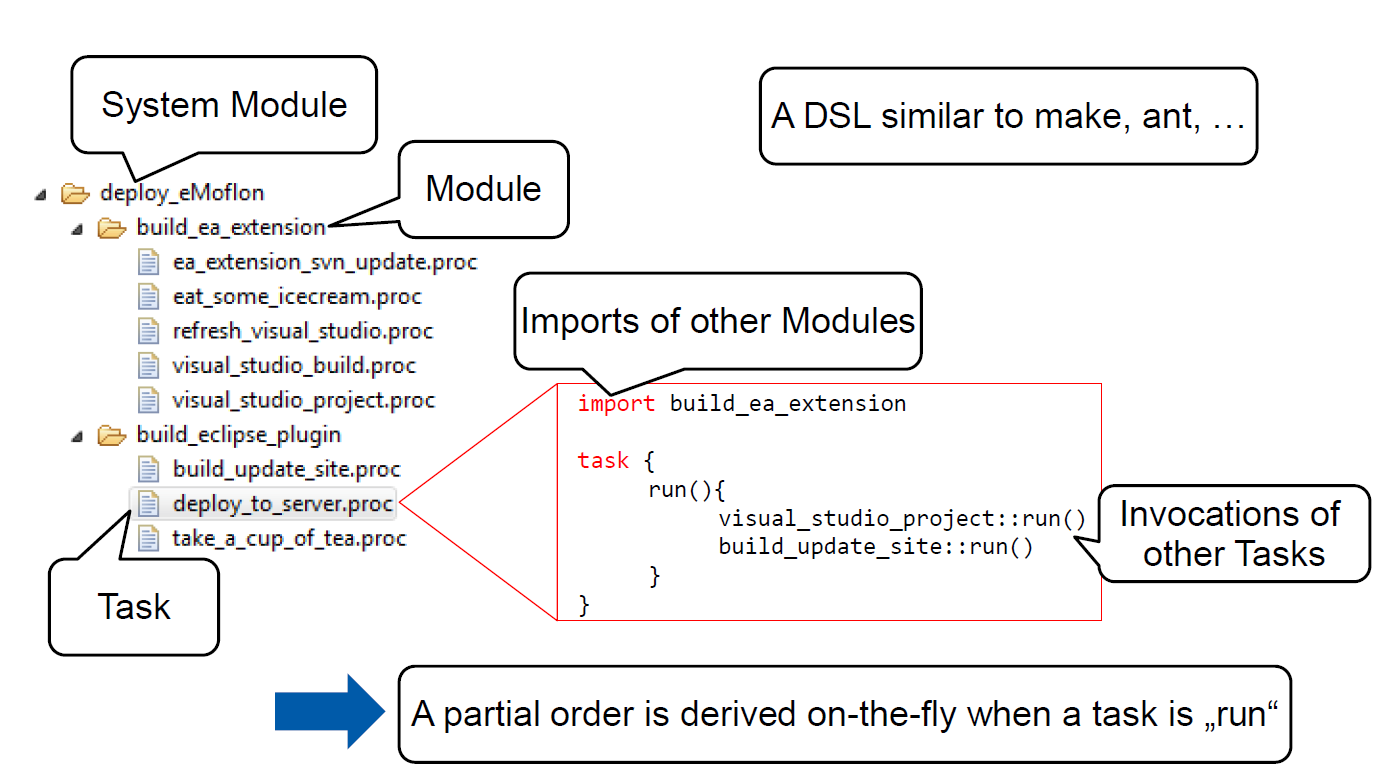
\includegraphics[width=0.5\textwidth]{figures/DSL.png} 
\end{center}
\caption{Example instance written in the DSL}
\label{fig: Example instance written in the DSL}
\end{figure}  

\subsection{The workflow for compiling and validating instances}
\label{sec: The workflow for compiling and validating instances}
The workflow for compiling and validating instances written in the DSL is depicted in Figure~\ref{fig: Workflow to Compile the DSL}.  


\begin{figure}[ht]
\begin{center} 
\includegraphics[width=0.5\textwidth]{figures/workflow.png} 
\end{center}
\caption{Workflow for compiling the DSL}
\label{fig: Workflow to Compile the DSL}
\end{figure}  




It consists of the following steps:
\begin{enumerate}[1)]
 \item \textbf{Text-to-Tree:}  The textual representation of an instance written in the DSL is parsed using a parser generated with ANTLR. The result is a tree representation of the instance. 
 \item \label{enumF2}\textbf{Tree-to-Model:} This tree is transformed to an instance of the Process Language metamodel using a transformation specified by a Triple Graph Grammar (TGG).
 \item \textbf{Model-to-Model:} Based on this representation (abstract syntax), the validation and (if necessary) correction operations are specified by Story Driven Modeling (SDM). Furthermore, the interpreter that runs the tasks in the defined order is specified here.
 \item \textbf{Model-to-Tree:} The corrected instances are transformed back to the tree representation using a transformation specified by the same TGG as used for the Tree-to-Model transformation.
 \item \textbf{Tree-to-Model:} Finally, the tree is unparsed using an unparser generated with ANTLR. 
\end{enumerate}




\subsection{Installation} 
Before you start, make sure that our tool eMoflon and ANTLR (a lexer parser generator) are installed.
Our tutorial\footnote{You can download the tutorial at \url{www.moflon.org}} contains detailed instructions on how to install eMoflon and set up ANTLR (see Chapter~2 and Chapter~5.1, respectively).



\subsection{Project Structure}
In order to facilitate the introduction into modeling with eMoflon, a workspace containing the basic building blocks can be downloaded\footnote{Eclipse Workspace: \url{http://www.moflon.org/fileadmin/download/eMoflon/ProcessLanguageWorkspace.zip}}. For example, it contains the parser and unparser and the sample instance presented in Figure \ref{fig: Example instance written in the DSL}, so that you can directly start with specifying SDMs and TGGs with eMoflon.

Open the workspace and take a look on the project structure. You find the following projects:
\begin{itemize}
  \item \textbf{ProcessLanguage}: The metamodel project containing the \texttt{.EAP} file, which is the link to our modeling frontend Enterprise Architect (EA). 
  \item\textbf{ProcessDefinition}: A repository project containing the Java code generated from the metamodel and from the SDM specification.
  \item \textbf{ProcessCodeAdapter}: The code adapter project (bidirectional Model-to-Text) contains the code generated from TGG.
\end{itemize}


To take a look at our frontend open Enterprise Architect by double clicking the \texttt{ProcessLanguage.eap} file located in the \texttt{ProcessLanguage} project. 
On the right-hand side, now you see a window labeled \textit{Project Browser} containing the \texttt{processLanguage} root package that consists of the following three packages:
\begin{itemize}
  \item \textbf{MocaTree}: containing the metamodel specification of the tree
  \item \textbf{ProcessCodeAdapter}: containing the TGG  
  \item \textbf{ProcessDefinition}: containing the metamodel specification (class diagram) of the \texttt{ProcessLanguage}, as well as the SDMs
\end{itemize}




